\documentclass[12pt]{article}
\usepackage[margin=1in]{geometry}
\usepackage{amsmath,amssymb,amsthm,mathtools}
\usepackage{booktabs,threeparttable,graphicx,setspace,enumitem,longtable,array}
\usepackage{xcolor}
\usepackage{etoolbox}
\AtBeginEnvironment{tabular}{\footnotesize}
\usepackage[authoryear,round]{natbib}
\usepackage[colorlinks=true,linkcolor=blue!50!black,citecolor=blue!50!black,urlcolor=blue!50!black]{hyperref}
\usepackage{fancyhdr}
\doublespacing
\emergencystretch=2em
\pagestyle{fancy}\fancyhf{}
\fancyhead[L]{\small Niroula and Niroula}
\fancyhead[R]{\small What Prices Reveal About Hidden Traders}
\fancyfoot[C]{\thepage}
\renewcommand{\headrulewidth}{0.3pt}
\setlength{\headheight}{14pt}

\newtheorem{theorem}{Theorem}[section]
\newtheorem{proposition}[theorem]{Proposition}
\newtheorem{lemma}[theorem]{Lemma}
\newtheorem{corollary}[theorem]{Corollary}
\theoremstyle{definition}
\newtheorem{definition}[theorem]{Definition}
\newtheorem{assumption}[theorem]{Assumption}
\theoremstyle{remark}
\newtheorem{remark}[theorem]{Remark}
\newcommand{\E}{\mathbb{E}}
\newcommand{\R}{\mathbb{R}}
\newcommand{\KL}{D_{\mathrm{KL}}}
\newcommand{\lab}[1]{\textsc{[#1]}}

\title{What Prices Reveal About Hidden Trader Populations,\\ and What Identifying Them Costs}
\author{Pratik Niroula\thanks{Department of Computer Information Science, Minnesota State University, Mankato, MN 56001, USA. \texttt{pratik.niroula@mnsu.edu}.}
\and Prashant Niroula\thanks{Faculty of Management, Tribhuvan University, Kirtipur, Nepal. \texttt{prashantniroula20@gmail.com}.}}
\date{This version: 30 October 2026}

\usepackage{array}
\begin{document}
\begin{center}\large Supplement to ``What Prices Reveal About Hidden Trader Populations, and What Identifying Them Costs'': a spectral blind spot and the measurement of reduced-form feedback\end{center}
\renewcommand{\thesection}{S\arabic{section}}\renewcommand{\thetable}{S\arabic{table}}\renewcommand{\thefigure}{S\arabic{figure}}\renewcommand{\theequation}{S\arabic{equation}}
These two analyses accompany the paper but are not needed for its main results.

\section{A spectral blind spot}\label{sec:blind}

Even without identification, could a supervisor monitor risk through eigenvalues or volatility?

\begin{theorem}[Spectral blindness]\label{thm:blind}
For any eigenvalues $0<\lambda_2<\lambda_1<1$, one-step price variance $s_1>0$ and stationary price variance $V$ large enough, there is a family of two-state markets $J_\theta=\begin{psmallmatrix}\lambda_1&\theta\\0&\lambda_2\end{psmallmatrix}$ with shock covariance ${\rm diag}(s_1,s_2(\theta))$ such that all members share the eigenvalues, the one-step price variance and the stationary price variance, while the worst-case transient gain $\sup_k\|e_1^\top J_\theta^k\|$ grows without bound in $\theta$.
\end{theorem}

\paragraph{In words.} Two markets can look identical by the usual risk measures, the same eigenvalues and the same price variance, and yet one of them can produce far larger losses in the short run. Monitoring eigenvalues or volatility alone therefore cannot certify that a market is safe.

At $\lambda=(0.8,0.7)$, $s_1=1$ and $V=5$, the gain is $1.77$, $5.10$, $16.95$, $50.85$ and $169.50$ for $\theta=1,3,10,30,100$, with stationary variance $5.000$ in every case; the cumulative gain rises from $18.3$ to $1{,}667.7$. No monitor that depends only on eigenvalues and second moments of the price can be uniformly safe (Figure~\ref{fig:blind}).

\begin{figure}[t]\centering
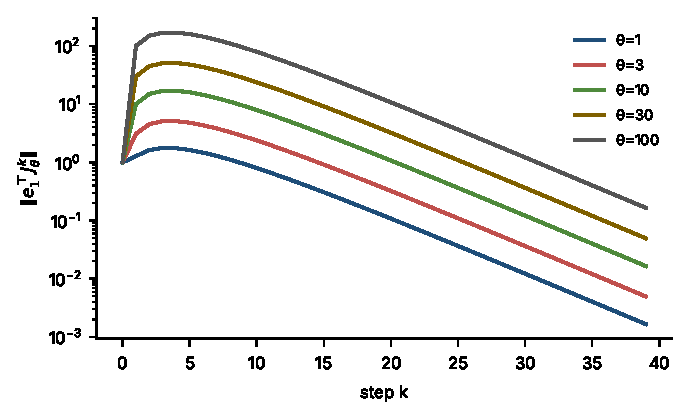
\includegraphics[width=0.6\textwidth]{figs/fig_blind.pdf}
\caption{Price-row transient gain of the spectral-blindness family $J_\theta$: eigenvalues $(0.8,0.7)$, one-step price variance 1 and stationary price variance 5 are the same for every $\theta$.}\label{fig:blind}
\end{figure}

Two clarifications prevent over-reading. First, the cohort economy of Section~2 is itself non-normal, yet its price output does not amplify (Lemma~2.3). Large weighted gains can be manufactured by output weights alone: with $C_w=(1,160)$, a price-and-memory functional peaks at $160.003$ at $t=0$, which is the static weight, not dynamic growth (Appendix~S3.5). Second, in a network of $M$ identical cohort economies coupled by symmetric nonnegative cross-impact, the coupled operator stays symmetric in the coordinates of Lemma~2.3; with cross-impact $0.05$, the spectral radius rises from $0.822$ ($M=1$) to $0.973$ ($M=10$) while the Kreiss constant stays at one, as it must for a stable symmetric operator (\texttt{recompute\_oct20.py}). A stable normal contraction cannot exhibit Euclidean state-norm transient growth. This does not exclude scalar input-output overshoot relative to initial impact, which also depends on the input and output maps. The positive-cohort no-overshoot result is model-specific; the companion paper studies a depth-depletion mechanism.
\section{Empirical feedback and its measurement}\label{sec:empirics}

The theory says what prices can reveal. The empirical work has two roles, and neither is a test of the identification bounds themselves, which concern controlled experiments no outside researcher can run. First, Section~6.4 tests the theory's policy prediction directly: that class-tagged data pin down memories that prices leave unrestricted. Second, this section asks what the reduced-form feedback indices a supervisor would compute from public data actually measure, and how much of them is feedback rather than filtering, timing or trading activity.

\subsection{Estimand and filtering mechanics}

In theory $x_t=p_t-p^*_t$ is the deviation from an unobserved fundamental. Empirical work replaces $p^*_t$ by a trailing filter. Let $p_b$ be a log price proxy on uniform bars of length $\Delta$ and $m_b=(1-\alpha)m_{b-1}+\alpha p_b$ an exponential moving average with $\alpha=2/(W/\Delta+1)$. The empirical state is
\begin{equation}\label{eq:ema}
x^{\rm EMA}_b\equiv p_b-m_b=(1-\alpha)(p_b-m_{b-1})=\frac{1-\alpha}{1-(1-\alpha)L}\Delta p_b .
\end{equation}

Because $x^{\rm EMA}_{b+1}=(1-\alpha)(p_{b+1}-m_b)$, a martingale price gives
\begin{equation}\label{eq:mech}
\E[x^{\rm EMA}_{b+1}\mid\mathcal F_b]=(1-\alpha)x^{\rm EMA}_b :
\end{equation}
the filtered state is an AR(1) with mechanical persistence $a_0=1-\alpha$, which equals $29/31\approx0.9355$ for $W=300$ seconds and $\Delta=10$ seconds.

Let $f_t$ be signed flow. The empirical VAR(1)
\begin{equation}\label{eq:var}
\begin{pmatrix}x^{\rm EMA}_{t+1}\\ f_{t+1}\end{pmatrix}=\begin{pmatrix}J_{11}&J_{12}\\ J_{21}&J_{22}\end{pmatrix}\begin{pmatrix}x^{\rm EMA}_t\\ f_t\end{pmatrix}+e_{t+1}
\end{equation}
has reduced-form coefficients, not authenticated impact or learner parameters. When denominators are nonzero we use the scale-invariant indices
\begin{equation}\label{eq:QS}
\hat Q=\frac{\hat J_{12}\hat J_{21}}{1-\hat J_{22}},\qquad\hat S=\hat J_{11}+\hat Q,\qquad\hat L=\frac{\hat Q}{1-\hat J_{11}} .
\end{equation}
Equation~\eqref{eq:mech} implies that $\hat J_{11}$ must be compared with $1-\alpha$, not with zero: persistence that a naive reading attributes to feedback can be pure filtering.

\subsection{Data}

\begin{table}[t]\centering\small
\begin{threeparttable}
\caption{Samples}\label{tab:samples}
\begin{tabular}{p{0.32\textwidth}p{0.25\textwidth}p{0.18\textwidth}l}
\toprule
Sample & Coverage & Size & Source\\
\midrule
Binance spot panel, 8 pairs & 96 dates, 2021--2024 & 66.3M one-second bars & Binance archive\\
Binance spot fee-event windows, 8 pairs & $\pm20$ days around 2022-07-08 and 2023-03-22 & 640 pair-days & Binance archive\\
Binance USD-M perpetuals, 30 symbols & 90 dates, 2023--2026 & 2{,}565 symbol-days & Binance archive\\
Binance BTCUSDT one-second panel & 72 dates, 2021--2023 & 6.2M one-second bars & Binance archive\\
Binance BTCUSDT noise-calibration days & January 10--20, 2023 & 11 days & Binance archive\\
\bottomrule
\end{tabular}
\begin{tablenotes}\footnotesize\item Binance files are verified against the published SHA-256 checksums (every file used). Sampled dates are the 10th and 24th of each month.\end{tablenotes}
\end{threeparttable}
\end{table}

\subsection{Clock alignment dominates reduced-form feedback}

We estimate \eqref{eq:var} on ten-second bars built from one-second Binance klines across a 96-date, eight-pair spot panel (the 10th and 24th of each month, 2021--2024) under three constructions (Table~\ref{tab:panel}), and run the identical pipeline on a placebo random walk with each pair-day's volatility. Pairing the state with \emph{next-bar} flow (a look-ahead) gives $\hat Q=0.0081$; aligning flow with the bar in which it is observed lowers this by more than an order of magnitude, to $0.00037$; and replacing the EMA state by raw returns gives an interval that includes zero. Mean $\hat J_{11}$ under observed flow is $0.9203$, below the mechanical $0.9355$, and the placebo reproduces the mechanical value ($0.9351$) with $\hat Q$ indistinguishable from zero. 

\begin{table}[t]\centering\small
\begin{threeparttable}
\caption{Multi-year Binance spot panel: reduced-form indices under three timing constructions}\label{tab:panel}
\setlength{\tabcolsep}{2.5pt}
\renewcommand{\arraystretch}{1.1}
\begin{tabular}{p{0.2\textwidth}ccccc}
\toprule
Construction & $\hat Q$ & Date interval & $\hat S$ & Date interval & $\hat Q>0$\\
\midrule
Forward-paired flow (look-ahead) & 0.0081424 & [0.0072965, 0.0089882] & 0.92074 & [0.91665, 0.92482] & 87.4\%\\
Observed-flow EMA & 0.0003733 & [0.0002351, 0.0005116] & 0.92072 & [0.91640, 0.92504] & 62.4\%\\
Observed, 30 flow lags & 0.0002580 & [0.0001415, 0.0003745] & 0.91738 & [0.91167, 0.92308] & 59.1\%\\
Observed raw return & $-$0.0001555 & [$-$0.0003732, 0.0000622] & $-$0.04051 & [$-$0.05078, $-$0.03025] & 49.2\%\\
Placebo random walk & 0.0000016 & [$-$0.0000020, 0.0000052] & 0.93510 & [0.93485, 0.93534] & 51.0\%\\
\bottomrule
\end{tabular}
\begin{tablenotes}\footnotesize\item 768 study units (96 dates $\times$ 8 pairs), 6{,}634{,}752 ten-second transitions; equal-weight asset means within date, then date means with Student intervals. Mechanical persistence $29/31=0.93548$. \end{tablenotes}
\end{threeparttable}
\end{table}

\begin{table}[t]\centering\small
\begin{threeparttable}
\caption{Asset means under forward-paired and observed flow}\label{tab:assets}
\begin{tabular}{lcccc}
\toprule
Pair & Forward-paired $\hat Q$ & Observed $\hat Q$ & $\hat Q_{30}$ & Observed $\hat S$\\
\midrule
BTC/USDT & 0.0141870 & 0.0006073 & 0.0004891 & 0.93464\\
ETH/USDT & 0.0130885 & 0.0005675 & 0.0002549 & 0.93511\\
SOL/USDT & 0.0087763 & 0.0002129 & 0.0001100 & 0.91966\\
ADA/USDT & 0.0067465 & 0.0003928 & 0.0003546 & 0.91452\\
DOGE/USDT & 0.0058956 & 0.0002464 & 0.0001432 & 0.92496\\
BNB/USDT & 0.0057420 & 0.0004479 & 0.0002762 & 0.89533\\
XRP/USDT & 0.0057034 & 0.0002249 & 0.0001508 & 0.92362\\
LTC/USDT & 0.0049997 & 0.0002870 & 0.0002853 & 0.91792\\
\bottomrule
\end{tabular}
\begin{tablenotes}\footnotesize\item 96 dates per pair. $\hat Q_{30}$ controls 30 ten-second bars of lagged flow. Placebo $|\hat Q|\le1.1\times10^{-5}$ for every pair. \end{tablenotes}
\end{threeparttable}
\end{table}



\subsection{Feedback beyond filtering mechanics}

We re-estimate feedback on a separate sample and add a placebo. We use Binance BTCUSDT one-second klines on 72 sampled days in 2021--2023. The state $x_t$ is the log price deviation from its EMA (span 30 one-second bins), $f_t$ is next-second signed taker flow, and a VAR(1) gives $\hat Q$. Because the filter alone produces persistence, we run the identical pipeline on a placebo: a random walk with the same one-second volatility, independent of the real flow.

\begin{table}[t]\centering
\begin{threeparttable}
\caption{Feedback beyond filtering mechanics (Binance BTCUSDT, 72 days, 2021--2023)}\label{tab:feedback}
\begin{tabular}{lcc}
\toprule
 & Real prices & Placebo (independent random walk)\\
\midrule
Mean loop gain $\hat Q$ & 0.0045 & 0.0000009\\
95\% CI (day bootstrap) & [0.0034, 0.0056] & [$-$0.0000006, 0.0000023]\\
Mean price persistence $\hat J_{11}$ & 0.9364 & 0.9357\\
Mechanical value $1-2/31$ & \multicolumn{2}{c}{0.9355}\\
\bottomrule
\end{tabular}
\begin{tablenotes}\footnotesize\item Placebo 95\% band across days: $[-0.0000095,0.0000156]$. This construction pairs the state with next-second flow; it is not comparable in level with the observed-flow ten-second index of Table~\ref{tab:panel}.\end{tablenotes}
\end{threeparttable}
\end{table}

Table~\ref{tab:feedback} gives two findings. Feedback, in the sense of a loop gain the filter cannot produce, is detectable: the real $\hat Q$ lies far outside the placebo band. It is also small, and the price persistence that a naive reading would attribute to feedback is almost entirely mechanical ($0.9364$ against $0.9355$). Because this construction pairs the state with next-second flow, part of $\hat Q$ reflects the timing effect of Table~\ref{tab:panel}; the placebo shows only that the filter does not produce it.

\subsection{Order splitting and the estimation of feedback}

Persistent order flow makes lagged-flow regressions inconsistent. Suppose flow follows $q_t=\gamma y_t+u_t$ with memory $y_t=(1-\eta)y_{t-1}+\eta\Delta p_{t-1}$, order splitting $u_t=\rho u_{t-1}+\nu_t$, and $\Delta p_t=\kappa q_t+\lambda z_t+e_t$ with an observed exogenous price shock $z_t$. Lagged returns are correlated with $u_{t-1}$, so OLS of flow on returns is biased even when $\gamma=0$. Quasi-differencing ($q_t-\rho q_{t-1}=\gamma(y_t-\rho y_{t-1})+\nu_t$) or instruments that move $y$ through prices but are independent of $u$ ($z_{t-1},z_{t-2},z_{t-3}$) restore consistency. We compare estimators over 500 replications with $\eta=0.3$ and $\rho=0.8$ (Table~\ref{tab:iv}).

\begin{table}[t]\centering
\begin{threeparttable}
\caption{Feedback estimators under order splitting (simulation, 500 replications)}\label{tab:iv}
\begin{tabular}{lcccc}
\toprule
Estimator & Coverage at $\gamma=0.2$ & Rejection at $\gamma=0$ & Bias & RMSE\\
\midrule
OLS & 0.000 & 1.000 & 0.892 & 0.893\\
Cochrane--Orcutt, true $\rho$ & 0.944 & 0.054 & 0.001 & 0.039\\
Cochrane--Orcutt, estimated $\rho$ & 0.916 & 0.080 & 0.002 & 0.043\\
2SLS & 0.938 & 0.044 & $-$0.002 & 0.116\\
LIML & 0.938 & 0.044 & $-$0.003 & 0.117\\
\bottomrule
\end{tabular}
\begin{tablenotes}\footnotesize\item Newey--West standard errors (10 lags), $T=3{,}000$. Median first-stage $F=224$; a placebo instrument (future $z$) has $F=0.62$. Estimators outside 93--97\% coverage give invalid inference. \end{tablenotes}
\end{threeparttable}
\end{table}

OLS is badly biased. Cochrane--Orcutt with the true $\rho$, 2SLS and LIML have correct size and coverage; Cochrane--Orcutt with an estimated $\rho$ under-covers \citep{cochrane1949,staiger1997}. These are properties of estimators in a simulated market. On real data, a 2024 sub-panel of 192 spot units shows why the correction matters little at our bar length: with one VAR lag, the flow-equation residuals have essentially no first-order serial correlation (median $\hat\rho=-0.0002$), and Cochrane--Orcutt quasi-differencing moves the mean loop gain from $3.15\times10^{-4}$ to $3.21\times10^{-4}$ (post hoc). Order splitting shows up instead at longer lags, which the 30-lag control of Table~\ref{tab:assets} addresses. A real-data instrumental-variables estimate needs an instrument whose exclusion can be defended, which we do not claim to have; funding-settlement times, for example, may affect order flow directly.

Controlling for 30 ten-second bars of lagged flow lowers $\hat Q$ further (Table~\ref{tab:assets}, column $\hat Q_{30}$), consistent with persistent order splitting.

\subsection{Feedback across 30 perpetual markets}

The companion paper estimates the same loop gain on one-minute bars of 30 Binance USD-M perpetuals spread across the liquidity ranking (2023--2024 training days). Measured feedback rises with depth: its Spearman correlation with log depth within 1\% of the mid is $+0.70$ [$0.41$, $0.87$], from about $0.012$ in BTCUSDT and ETHUSDT to $0.0016$ on average in the thinnest third, and the placebo pipeline gives $\hat Q\approx0$ for every symbol. Feedback in this reduced-form sense is a feature of deep, algorithmically traded books.

\subsection{Two fee events}

Binance set spot trading fees on BTC pairs to zero on July 8, 2022 and reinstated them on March 22, 2023. Each event changes the cost of trading BTCUSDT while leaving the seven other pairs unchanged, and the second reverses the first. For every pair and every day within 20 days of each event we compute daily quote volume and the observed-flow $\hat Q$, and estimate $Y_{it}=\alpha_i+\gamma_t+\beta\,{\rm ZeroFee}_{it}+e_{it}$ with pair and date fixed effects and date-clustered errors, separately for each event and pooled (Table~\ref{tab:fee2}).

\begin{table}[t]\centering\small
\begin{threeparttable}
\caption{Zero fees on BTCUSDT: activity and measured feedback}\label{tab:fee2}
\begin{tabular}{lccc}
\toprule
 & Zero fees introduced & Zero fees removed & Pooled\\
 & (2022-07-08) & (2023-03-22) & \\
\midrule
Log quote volume, $\hat\beta$ & 0.945 (0.074) & 1.599 (0.080) & 1.272 (0.084)\\
Observed-flow $\hat Q$, $\hat\beta$ & 0.00058 (0.00032) & $-$0.00091 (0.00060) & $-$0.00016 (0.00036)\\
\quad $p$-value & 0.078 & 0.140 & 0.650\\
Pair-days & 320 & 320 & 640\\
\bottomrule
\end{tabular}
\begin{tablenotes}\footnotesize\item $\hat\beta$ is the effect of zero fees on BTCUSDT relative to seven control pairs; date-clustered standard errors in parentheses. For the second event ZeroFee equals one before March 22, 2023. \end{tablenotes}
\end{threeparttable}
\end{table}

The fee change moved activity enormously: zero fees multiplied BTCUSDT volume relative to the controls by $e^{0.945}\approx2.6$ when they began, and their removal divided it by $e^{1.599}\approx4.9$. Measured feedback did not follow. The two point estimates have opposite signs, neither is significant, and the pooled effect is $-0.00016$ with an interval of $[-0.00087,0.00055]$, against a sample mean of $0.00037$. A strong first stage with no second-stage response says that $\hat Q$ is not a by-product of trading activity, and the reversal design removes the main weakness of a single treated event. With one treated asset the interval remains wide, so this is evidence that $\hat Q$ does not scale with activity, not a proof of invariance.


\begin{thebibliography}{99}\setlength{\itemsep}{2pt}\small
\bibitem[Alfonsi et~al.(2012)]{alfonsi2012} Alfonsi, A., A. Schied, and A. Slynko (2012). Order book resilience, price manipulation, and the positive portfolio problem. \emph{SIAM Journal on Financial Mathematics} 3. doi:10.1137/110822098.
\bibitem[Alfonsi et~al.(2016)]{alfonsi2016} Alfonsi, A., A. Schied, and F. Kl\"ock (2016). Multivariate transient price impact and matrix-valued positive definite functions. \emph{Mathematics of Operations Research} 41, 914--934.
\bibitem[Almgren and Chriss(2001)]{almgren2001} Almgren, R., and N. Chriss (2001). Optimal execution of portfolio transactions. \emph{Journal of Risk} 3, 5--39.
\bibitem[Barberis et~al.(2015)]{barberis2015} Barberis, N., R. Greenwood, L. Jin, and A. Shleifer (2015). X-CAPM: An extrapolative capital asset pricing model. \emph{Journal of Financial Economics} 115, 1--24.
\bibitem[Barberis et~al.(2018)]{barberis2018} Barberis, N., R. Greenwood, L. Jin, and A. Shleifer (2018). Extrapolation and bubbles. \emph{Journal of Financial Economics} 129, 203--227.
\bibitem[Biais et~al.(2015)]{biais2015} Biais, B., T. Foucault, and S. Moinas (2015). Equilibrium fast trading. \emph{Journal of Financial Economics} 116, 292--313.
\bibitem[Crouzet et~al.(2020)]{crouzet2020} Crouzet, N., I. Dew-Becker, and C.\,G. Nathanson (2020). On the effects of restricting short-term investment. \emph{Review of Financial Studies} 33, 1--43.
\bibitem[Cespa and Vives(2015)]{cespa2015} Cespa, G., and X. Vives (2015). The beauty contest and short-term trading. \emph{Journal of Finance} 70, 2099--2154.
\bibitem[Amilon(2008)]{amilon2008} Amilon, H. (2008). Estimation of an adaptive stock market model with heterogeneous agents. \emph{Journal of Empirical Finance} 15, 342--362.
\bibitem[Batenkov et~al.(2021)]{batenkov2021} Batenkov, D., G. Goldman, and Y. Yomdin (2021). Super-resolution of near-colliding point sources. \emph{Information and Inference} 10, 515--572.
\bibitem[Bernstein(1914)]{bernstein1914} Bernstein, S. (1914). Sur la meilleure approximation de $|x|$ par des polyn\^omes de degr\'es donn\'es. \emph{Acta Mathematica} 37, 1--57.
\bibitem[Bessembinder et~al.(2006)]{bessembinder2006} Bessembinder, H., W. Maxwell, and K. Venkataraman (2006). Market transparency, liquidity externalities, and institutional trading costs in corporate bonds. \emph{Journal of Financial Economics} 82, 251--288.
\bibitem[Boehmer et~al.(2005)]{boehmer2005} Boehmer, E., G. Saar, and L. Yu (2005). Lifting the veil: An analysis of pre-trade transparency at the NYSE. \emph{Journal of Finance} 60, 783--815.
\bibitem[Bouchaud et~al.(2004)]{bouchaud2004} Bouchaud, J.-P., Y. Gefen, M. Potters, and M. Wyart (2004). Fluctuations and response in financial markets: The subtle nature of ``random'' price changes. \emph{Quantitative Finance} 4, 176--190.
\bibitem[Bouchaud et~al.(2018)]{bouchaud2018} Bouchaud, J.-P., J. Bonart, J. Donier, and M. Gould (2018). \emph{Trades, Quotes and Prices: Financial Markets Under the Microscope}. Cambridge University Press.
\bibitem[Brock and Hommes(1998)]{brock1998} Brock, W.~A., and C.~H. Hommes (1998). Heterogeneous beliefs and routes to chaos in a simple asset pricing model. \emph{Journal of Economic Dynamics and Control} 22, 1235--1274.
\bibitem[Brogaard et~al.(2014)]{brogaard2014} Brogaard, J., T. Hendershott, and R. Riordan (2014). High-frequency trading and price discovery. \emph{Review of Financial Studies} 27, 2267--2306.
\bibitem[Brunnermeier and Pedersen(2009)]{brunnermeier2009} Brunnermeier, M. K., and L. H. Pedersen (2009). Market liquidity and funding liquidity. \emph{Review of Financial Studies} 22, 2201--2238.
\bibitem[Castelli and Cover(1996)]{castelli1996} Castelli, V., and T.~M. Cover (1996). The relative value of labeled and unlabeled samples in pattern recognition with an unknown mixing parameter. \emph{IEEE Transactions on Information Theory} 42, 2102--2117.
\bibitem[Cochrane and Orcutt(1949)]{cochrane1949} Cochrane, D., and G. H. Orcutt (1949). Application of least squares regression to relationships containing auto-correlated error terms. \emph{Journal of the American Statistical Association} 44, 32--61.
\bibitem[Colliard et~al.(2022)]{colliard2022} Colliard, J.-E., T. Foucault, and S. Lovo (2022). Algorithmic pricing and liquidity in securities markets. CEPR Discussion Paper 17606.
\bibitem[Banerjee and Szydlowski(2026)]{banerjee2026} Banerjee, S., and M. Szydlowski (2026). Trading against algorithms: Price dynamics and risk-sharing in a market with Q-learners. Working paper.
\bibitem[Moallemi et~al.(2008)]{moallemi2008} Moallemi, C.~C., B. Park, and B. Van Roy (2008). Strategic execution in the presence of an uninformed arbitrageur. arXiv preprint arXiv:0801.3001.
\bibitem[Tremacoldi-Rossi(2025)]{tremacoldi2025} Tremacoldi-Rossi, P. (2025). Manipulating algorithmic markets. Working paper.
\bibitem[Trebbi et~al.(2024)]{trebbi2024} Trebbi, F., M.~B. Zhang, and M. Simkovic (2024). The cost of regulatory compliance in the United States. Working paper.
\bibitem[van Waarde et~al.(2020)]{vanwaarde2020} van Waarde, H.~J., J. Eising, H.~L. Trentelman, and M.~K. Camlibel (2020). Data informativity: A new perspective on data-driven analysis and control. \emph{IEEE Transactions on Automatic Control} 65, 4753--4768.
\bibitem[Dou et~al.(2025)]{dou2025} Dou, W.~W., I. Goldstein, and Y. Ji (2025). AI-powered trading, algorithmic collusion, and price efficiency. NBER Working Paper 34054.
\bibitem[Duarte and Young(2009)]{duarte2009} Duarte, J., and L. Young (2009). Why is PIN priced? \emph{Journal of Financial Economics} 91, 119--138.
\bibitem[Easley et~al.(1996)]{easley1996} Easley, D., N.~M. Kiefer, M. O'Hara, and J.~B. Paperman (1996). Liquidity, information, and infrequently traded stocks. \emph{Journal of Finance} 51, 1405--1436.
\bibitem[European Commission(2017)]{rts24} European Commission (2017). Commission Delegated Regulation (EU) 2017/580 of 24 June 2016 supplementing Regulation (EU) No 600/2014 with regard to regulatory technical standards for the maintenance of relevant data relating to orders in financial instruments (RTS 24), Article 2(1)(b)--(c). \emph{Official Journal of the European Union} L 87, 31.3.2017.
\bibitem[European Commission(2017b)]{rts6} European Commission (2017). Commission Delegated Regulation (EU) 2017/589 of 19 July 2016 supplementing Directive 2014/65/EU with regard to regulatory technical standards specifying the organisational requirements of investment firms engaged in algorithmic trading (RTS 6). \emph{Official Journal of the European Union} L 87, 31.3.2017.
\bibitem[ESMA(2016)]{esma2016} European Securities and Markets Authority (2016). Guidelines on transaction reporting, order record keeping and clock synchronisation under MiFID II. ESMA/2016/1452.
\bibitem[Fan(1991)]{fan1991} Fan, J. (1991). On the optimal rates of convergence for nonparametric deconvolution problems. \emph{Annals of Statistics} 19, 1257--1272.
\bibitem[Leach and Madhavan(1993)]{leach1993} Leach, J.\,C., and A.\,N. Madhavan (1993). Price experimentation and security market structure. \emph{Review of Financial Studies} 6, 375--404.

\bibitem[Andrews and Cheng(2012)]{andrews2012} Andrews, D.\,W.\,K., and X. Cheng (2012). Estimation and inference with weak, semi-strong, and strong identification. \emph{Econometrica} 80, 2153--2211.

\bibitem[Barth and Kahn(2021)]{barth2021} Barth, D., and R.\,J. Kahn (2021). Hedge funds and the Treasury cash-futures disconnect. Office of Financial Research Working Paper 21-01.

\bibitem[Forssell and Ljung(1999)]{forssell1999} Forssell, U., and L. Ljung (1999). Closed-loop identification revisited. \emph{Automatica} 35, 1215--1241.
\bibitem[Franke and Westerhoff(2012)]{franke2012} Franke, R., and F. Westerhoff (2012). Structural stochastic volatility in asset pricing dynamics: Estimation and model contest. \emph{Journal of Economic Dynamics and Control} 36, 1193--1211.
\bibitem[Gatheral(2010)]{gatheral2010} Gatheral, J. (2010). No-dynamic-arbitrage and market impact. \emph{Quantitative Finance} 10, 749--759.
\bibitem[Glosten and Milgrom(1985)]{glosten1985} Glosten, L. R., and P. R. Milgrom (1985). Bid, ask and transaction prices in a specialist market with heterogeneously informed traders. \emph{Journal of Financial Economics} 14, 71--100.
\bibitem[Hasbrouck(1991)]{hasbrouck1991} Hasbrouck, J. (1991). Measuring the information content of stock trades. \emph{Journal of Finance} 46, 179--207.
\bibitem[Heinrich and Kahn(2018)]{heinrich2018} Heinrich, P., and J. Kahn (2018). Strong identifiability and optimal minimax rates for finite mixture estimation. \emph{Annals of Statistics} 46, 2844--2870.
\bibitem[Hendershott et~al.(2011)]{hendershott2011} Hendershott, T., C.~M. Jones, and A.~J. Menkveld (2011). Does algorithmic trading improve liquidity? \emph{Journal of Finance} 66, 1--33.
\bibitem[Hua and Sarkar(1990)]{hua1990} Hua, Y., and T. K. Sarkar (1990). Matrix pencil method for estimating parameters of exponentially damped/undamped sinusoids in noise. \emph{IEEE Transactions on Acoustics, Speech, and Signal Processing} 38, 814--824.
\bibitem[Katz et~al.(2023)]{katz2023} Katz, R., N. Diab, and D. Batenkov (2023). On the accuracy of Prony's method for recovery of exponential sums with closely spaced exponents. arXiv preprint arXiv:2302.05883.
\bibitem[Kirilenko et~al.(2017)]{kirilenko2017} Kirilenko, A., A. S. Kyle, M. Samadi, and T. Tuzun (2017). The Flash Crash: High-frequency trading in an electronic market. \emph{Journal of Finance} 72, 967--998.
\bibitem[Kong and Valiant(2017)]{kong2017} Kong, W., and G. Valiant (2017). Spectrum estimation from samples. \emph{Annals of Statistics} 45, 2218--2247.
\bibitem[Kreiss(1962)]{kreiss1962} Kreiss, H.-O. (1962). \"Uber die Stabilit\"atsdefinition f\"ur Differenzengleichungen die partielle Differentialgleichungen approximieren. \emph{BIT Numerical Mathematics} 2, 153--181.
\bibitem[Kukacka and Barunik(2017)]{kukacka2017} Kukacka, J., and J. Barunik (2017). Estimation of financial agent-based models with simulated maximum likelihood. \emph{Journal of Economic Dynamics and Control} 85, 21--45.
\bibitem[Kyle(1985)]{kyle1985} Kyle, A. S. (1985). Continuous auctions and insider trading. \emph{Econometrica} 53, 1315--1335.
\bibitem[Le Cam(1986)]{lecam1986} Le Cam, L. (1986). \emph{Asymptotic Methods in Statistical Decision Theory}. Springer.
\bibitem[Liu and Ammari(2022)]{liu2023} Liu, P., and H. Ammari (2022). Super-resolution of positive near-colliding point sources. arXiv preprint arXiv:2212.00536.
\bibitem[Ljung(1999)]{ljung1999} Ljung, L. (1999). \emph{System Identification: Theory for the User}, 2nd ed. Prentice Hall, Upper Saddle River, NJ.
\bibitem[Makarov and Schoar(2020)]{makarov2020} Makarov, I., and A. Schoar (2020). Trading and arbitrage in cryptocurrency markets. \emph{Journal of Financial Economics} 135, 293--319.
\bibitem[Manole and Ho(2022)]{manole2022} Manole, T., and N. Ho (2022). Refined convergence rates for maximum likelihood estimation under finite mixture models. \emph{Proceedings of the 39th International Conference on Machine Learning}, PMLR 162.
\bibitem[Manski(2003)]{manski2003} Manski, C.~F. (2003). \emph{Partial Identification of Probability Distributions}. Springer, New York.
\bibitem[Niroula et~al.(2026)]{niroula2026b} Niroula, P., S. Alkhushayni, Y. Chen, M. Bhavsar, and P. Niroula (2026). From human markets to machine markets: Transient amplification, an exact depth condition, and a maximal pre-trade guard. Working paper, Minnesota State University, Mankato.
\bibitem[Moitra(2015)]{moitra2015} Moitra, A. (2015). Super-resolution, extremal functions and the condition number of Vandermonde matrices. In \emph{Proceedings of the 47th Annual ACM Symposium on Theory of Computing (STOC)}, 821--830.
\bibitem[Moskowitz et~al.(2012)]{moskowitz2012} Moskowitz, T. J., Y. H. Ooi, and L. H. Pedersen (2012). Time series momentum. \emph{Journal of Financial Economics} 104, 228--250.
\bibitem[Obizhaeva and Wang(2013)]{obizhaeva2013} Obizhaeva, A. A., and J. Wang (2013). Optimal trading strategy and supply/demand dynamics. \emph{Journal of Financial Markets} 16, 1--32.
\bibitem[Pagano and R\"oell(1996)]{pagano1996} Pagano, M., and A. R\"oell (1996). Transparency and liquidity: A comparison of auction and dealer markets with informed trading. \emph{Journal of Finance} 51, 579--611.
\bibitem[Park and Van Roy(2015)]{parkvanroy2015} Park, B., and B. Van Roy (2015). Adaptive execution: Exploration and learning of price impact. \emph{Operations Research}, doi:10.1287/opre.2015.1415.
\bibitem[Rebafka and Roueff(2015)]{rebafka2015} Rebafka, T., and F. Roueff (2015). Nonparametric estimation of the mixing density using polynomials. arXiv preprint arXiv:1002.4516.
\bibitem[Rivlin(1981)]{rivlin1981} Rivlin, T. J. (1981). \emph{An Introduction to the Approximation of Functions}. Dover.
\bibitem[Roll(1984)]{roll1984} Roll, R. (1984). A simple implicit measure of the effective bid-ask spread in an efficient market. \emph{Journal of Finance} 39, 1127--1139.
\bibitem[Roy and Kailath(1989)]{roy1989} Roy, R., and T. Kailath (1989). ESPRIT---estimation of signal parameters via rotational invariance techniques. \emph{IEEE Transactions on Acoustics, Speech, and Signal Processing} 37, 984--995.
\bibitem[CAT LLC(2026)]{catbudget2026} Consolidated Audit Trail, LLC (2026). Consolidated Audit Trail, LLC 2026 Financial and Operating Budget, 31 March 2026 (total expenses \$147{,}044{,}869). \url{https://www.catnmsplan.com/cat-financial-and-operating-budget}.
\bibitem[SEC(2010)]{sec2010} U.S. Securities and Exchange Commission (2010). Risk management controls for brokers or dealers with market access. Release No.\ 34-63241.
\bibitem[SEC(2012)]{sec2012} U.S. Securities and Exchange Commission (2012). Consolidated Audit Trail; Final Rule (Release No.\ 34-67457, July 18, 2012, 77 FR 45722 at 45790--45795, pp.\ 220--238; proposing release No.\ 34-62174, May 26, 2010, 75 FR 32556 at 32598, 32600, pp.\ 147, 153).
\bibitem[SEC(2016)]{sec2016} U.S. Securities and Exchange Commission (2016). Joint Industry Plan; Order Approving the National Market System Plan Governing the Consolidated Audit Trail. Release No.\ 34-79318, November 15, 2016, 81 FR 84696 at 84801, p.\ 363.
\bibitem[SEC(2024)]{sec2024cat} U.S. Securities and Exchange Commission (2024). Notice of Filing of Proposed Rule Change Relating to the 2025 CAT Budget. Release No.\ 34-101901, December 12, 2024, p.\ 4 (revised May 2025).
\bibitem[SEC(2025)]{sec2025} U.S. Securities and Exchange Commission (2025). Order granting exemptive relief from certain requirements of the National Market System Plan governing the Consolidated Audit Trail. Release No.\ 34-102386, February 10, 2025.
\bibitem[Shahram and Milanfar(2005)]{shahram2005} Shahram, M., and P. Milanfar (2005). On the resolvability of sinusoids with nearby frequencies in the presence of noise. \emph{IEEE Transactions on Signal Processing} 53, 2579--2588.
\bibitem[Shleifer and Vishny(1992)]{shleifer1992} Shleifer, A., and R. W. Vishny (1992). Liquidation values and debt capacity: A market equilibrium approach. \emph{Journal of Finance} 47, 1343--1366.
\bibitem[Sornette et~al.(2023)]{sornette2023} Sornette, D., S. Lera, J. Lin, and K. Wu (2023). Non-normal interactions create socio-economic bubbles. \emph{Communications Physics} 6, 261.
\bibitem[Staiger and Stock(1997)]{staiger1997} Staiger, D., and J. H. Stock (1997). Instrumental variables regression with weak instruments. \emph{Econometrica} 65, 557--586.
\bibitem[Trefethen and Embree(2005)]{trefethen2005} Trefethen, L. N., and M. Embree (2005). \emph{Spectra and Pseudospectra: The Behavior of Nonnormal Matrices and Operators}. Princeton University Press.
\bibitem[Tsybakov(2009)]{tsybakov2009} Tsybakov, A. B. (2009). \emph{Introduction to Nonparametric Estimation}. Springer.
\bibitem[Varga and Carpenter(1985)]{varga1985} Varga, R. S., and A. J. Carpenter (1985). On the Bernstein conjecture in approximation theory. \emph{Constructive Approximation} 1, 333--348.
\bibitem[Wagenmaker and Jamieson(2020)]{wagenmaker2020} Wagenmaker, A., and K. Jamieson (2020). Active learning for identification of linear dynamical systems. In \emph{Proceedings of the 33rd Conference on Learning Theory}, PMLR 125, 3487--3582.
\bibitem[Wagenmaker et~al.(2021)]{wagenmaker2021} Wagenmaker, A.~J., M. Simchowitz, and K. Jamieson (2021). Task-optimal exploration in linear dynamical systems. In \emph{Proceedings of the 38th International Conference on Machine Learning}, PMLR 139, 10641--10652.
\bibitem[Wellman(2006)]{wellman2006} Wellman, M.~P. (2006). Methods for empirical game-theoretic analysis. In \emph{Proceedings of the 21st National Conference on Artificial Intelligence (AAAI-06)}, 1552--1555.
\bibitem[Whittle(1953)]{whittle1953} Whittle, P. (1953). Estimation and information in stationary time series. \emph{Arkiv f\"or Matematik} 2, 423--434.
\bibitem[Wu and Yang(2020)]{wu2020} Wu, Y., and P. Yang (2020). Optimal estimation of Gaussian mixtures via denoised method of moments. \emph{Annals of Statistics} 48, 1981--2007.
\end{thebibliography}
\end{document}
